% 图 3.4 八面体与四面体环境中的晶体场劈裂（自由离子五重简并 -> eg/t2g）
\documentclass[tikz,border=5pt]{standalone}
\usetikzlibrary{arrows.meta}
\usepackage{amsmath}
\usepackage{bm}
\usepackage{fontspec}
\setmainfont{Times New Roman}
\begin{document}
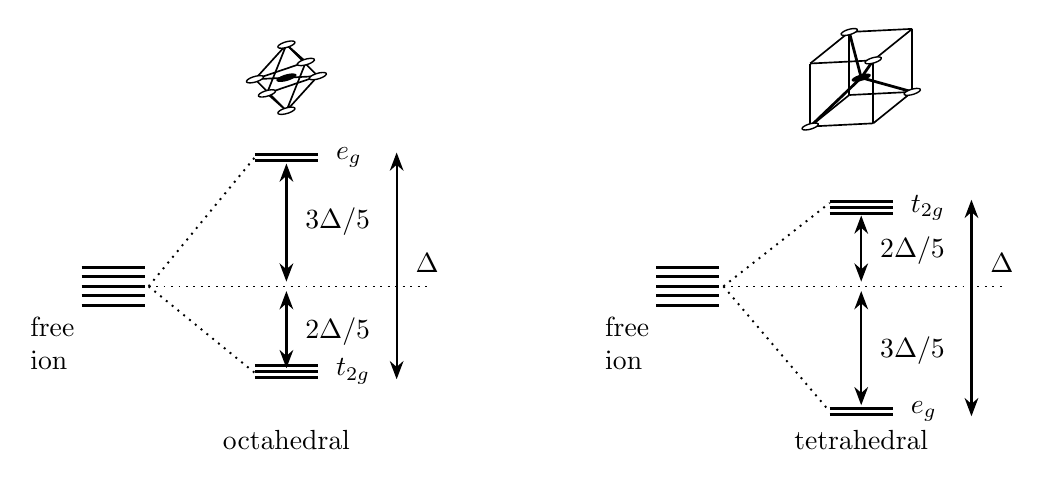
\begin{tikzpicture}[line width=0.8pt,>=Stealth,
  lvl/.style={line width=1.1},
  fan/.style={line width=0.7,dotted},
  darr/.style={<->,{Stealth[]}-{Stealth[]}}]
% ================ 左半：octahedral ================
\begin{scope}
% 自由离子五条简并能级
\foreach \i in {0,...,4}{\draw[lvl] (0.15,0.24-0.12*\i) -- (0.95,0.24-0.12*\i);}
\node[anchor=north west,align=left,inner sep=1pt] at (-0.55,-0.34) {free\\ion};
% 点线扇形展开 + 重心参考线
\draw[fan] (1.0,0) -- (2.35,1.64);
\draw[fan] (1.0,0) -- (2.35,-1.10);
\draw[fan,line width=0.5] (1.0,0) -- (4.6,0);
% e_g（二重，上方）
\draw[lvl] (2.35,1.60) -- (3.15,1.60);
\draw[lvl] (2.35,1.68) -- (3.15,1.68);
\node[anchor=west] at (3.25,1.64) {$e_g$};
% t_2g（三重，下方）
\draw[lvl] (2.35,-1.00) -- (3.15,-1.00);
\draw[lvl] (2.35,-1.08) -- (3.15,-1.08);
\draw[lvl] (2.35,-1.16) -- (3.15,-1.16);
\node[anchor=west] at (3.25,-1.08) {$t_{2g}$};
% 劈裂双箭头
\draw[darr] (2.75,0.06) -- (2.75,1.56);
\node[anchor=west] at (2.86,0.82) {$3\Delta/5$};
\draw[darr] (2.75,-0.06) -- (2.75,-1.04);
\node[anchor=west] at (2.86,-0.58) {$2\Delta/5$};
% 总劈裂 Δ
\draw[darr] (4.15,-1.18) -- (4.15,1.70);
\node[anchor=west] at (4.26,0.30) {$\Delta$};
% 顶部小八面体图标
\begin{scope}[shift={(2.75,2.65)},scale=0.42,x={(-0.62cm,-0.50cm)},y={(1cm,0.05cm)},z={(0,1cm)}]
\draw[line width=0.6]
  (0,0,1) -- (0,0.95,0) -- (0.95,0,0) -- (0,0,-1) -- (0,-0.95,0) -- (-0.95,0,0) -- cycle;
\draw[line width=0.6] (0,0,1) -- (0.95,0,0) (0,0,1) -- (-0.95,0,0)
  (0,0,1) -- (0,-0.95,0) (0,0,-1) -- (0,0.95,0)
  (0,0,-1) -- (-0.95,0,0) (0,0.95,0) -- (0,-0.95,0);
\filldraw[fill=white,line width=0.5] (0,0,1) circle (0.22);
\filldraw[fill=white,line width=0.5] (0,0,-1) circle (0.22);
\filldraw[fill=white,line width=0.5] (0,0.95,0) circle (0.22);
\filldraw[fill=white,line width=0.5] (0,-0.95,0) circle (0.22);
\filldraw[fill=white,line width=0.5] (0.95,0,0) circle (0.22);
\filldraw[fill=white,line width=0.5] (-0.95,0,0) circle (0.22);
\fill (0,0,0) circle (0.26);
\end{scope}
\node at (2.75,-1.95) {octahedral};
\end{scope}
% ================ 右半：tetrahedral ================
\begin{scope}[shift={(7.3,0)}]
\foreach \i in {0,...,4}{\draw[lvl] (0.15,0.24-0.12*\i) -- (0.95,0.24-0.12*\i);}
\node[anchor=north west,align=left,inner sep=1pt] at (-0.55,-0.34) {free\\ion};
\draw[fan] (1.0,0) -- (2.35,1.06);
\draw[fan] (1.0,0) -- (2.35,-1.59);
\draw[fan,line width=0.5] (1.0,0) -- (4.6,0);
% t_2g（三重，上方，距重心 2Δ/5）
\draw[lvl] (2.35,0.92) -- (3.15,0.92);
\draw[lvl] (2.35,1.00) -- (3.15,1.00);
\draw[lvl] (2.35,1.08) -- (3.15,1.08);
\node[anchor=west] at (3.25,1.00) {$t_{2g}$};
% e_g（二重，下方，距重心 3Δ/5）
\draw[lvl] (2.35,-1.55) -- (3.15,-1.55);
\draw[lvl] (2.35,-1.63) -- (3.15,-1.63);
\node[anchor=west] at (3.25,-1.59) {$e_g$};
\draw[darr] (2.75,0.06) -- (2.75,0.90);
\node[anchor=west] at (2.86,0.46) {$2\Delta/5$};
\draw[darr] (2.75,-0.06) -- (2.75,-1.51);
\node[anchor=west] at (2.86,-0.82) {$3\Delta/5$};
\draw[darr] (4.15,-1.65) -- (4.15,1.10);
\node[anchor=west] at (4.26,0.30) {$\Delta$};
% 顶部小立方体图标
\begin{scope}[shift={(2.75,2.65)},scale=0.40,x={(-0.62cm,-0.50cm)},y={(1cm,0.05cm)},z={(0,1cm)}]
\foreach \a in {-1,1}{\foreach \b in {-1,1}{
  \draw[line width=0.6] (\a,\b,-1) -- (\a,\b,1);
  \draw[line width=0.6] (\a,-1,\b) -- (\a,1,\b);
  \draw[line width=0.6] (-1,\a,\b) -- (1,\a,\b);
}}
\draw[line width=1.0] (0,0,0) -- (1,1,1);
\draw[line width=1.0] (0,0,0) -- (1,-1,-1);
\draw[line width=1.0] (0,0,0) -- (-1,1,-1);
\draw[line width=1.0] (0,0,0) -- (-1,-1,1);
\filldraw[fill=white,line width=0.5] (1,1,1) circle (0.22);
\filldraw[fill=white,line width=0.5] (1,-1,-1) circle (0.22);
\filldraw[fill=white,line width=0.5] (-1,1,-1) circle (0.22);
\filldraw[fill=white,line width=0.5] (-1,-1,1) circle (0.22);
\fill (0,0,0) circle (0.26);
\end{scope}
\node at (2.75,-1.95) {tetrahedral};
\end{scope}
\end{tikzpicture}
\end{document}
